\documentclass[a4paper,twoside,10pt]{report}
\usepackage[english]{babel}
\usepackage[utf8]{inputenc}
\usepackage{graphicx}
\usepackage{url}
\usepackage[export]{adjustbox}
\usepackage{indentfirst}
% pdflatex

% redefinição das margens das páginas
\setlength{\textheight}{24.00cm}
\setlength{\textwidth}{15.50cm}
\setlength{\topmargin}{0.35cm}
\setlength{\headheight}{0cm}
\setlength{\headsep}{0cm}
\setlength{\oddsidemargin}{0.25cm}
\setlength{\evensidemargin}{0.25cm}

\begin{document}

\begin{figure}[t]
\resizebox{60mm}{!}{
\includegraphics[left]{logoISEL.png}}
\end{figure}

\title{\huge\textbf{Lean Dashboard}}

\author{
\begin{tabular}{c}
José Pedro Jesus, n.º 44805\\
Hugo Manuel Jacinto Pinheiro, n.º 44886\\
Tomás Simão Mendes dos Santos, n.º 45363\\
\end{tabular}
}

\date{
\begin{tabular}{ll}
  {\textbf{Orientadores:}} & João Pereira, e-mail: joao.pereira@inetum.world, Inetum \\
                 & Filipe Freitas, e-mail: ffreitas@cc.isel.ipl.pt\\
\end{tabular}\\
\vspace{5mm}
\textbf{June 6th 2021 - V1 }}


\maketitle

\title{\huge\textbf{Abstract}}
\\ \newline
*O abstract será feito posteriormente*


\pagebreak
\tableofcontents{}
\newpage


\chapter{Introduction}

\section{Background}
Nowadays, within a company, it is even more important to have an organized and cooperative team with knowledge of all the steps and goals that need to be worked on for the various projects they are currently participating in.
Each member of the team must keep track of high amounts of information and since it is not uncommon that when working on a project a couple of platforms are used to keep track and share work done by the various members, useful information can be scattered on a vast amount of platforms, and sometimes even inside a single platform.
The information relative to a project can be obtained from different sources and it is all aggregated in one place, readily available to be displayed to a work team to better guide a certain project's development.

\section{Relevancy}
The Lean Dashboard Project will be developed to help the company's workers keeping track of all the possible tasks for their projects, gathering all the information needed for the various activities from the many sources that are necessary, presenting it on an easy to read and reactive web application.
The project at hands will be developed in partnership with Inetum\cite{INETUM} and will centre around the development of a responsive web application capable of running on a multitude of devices, ranging from smartphones to desktop computers to large screens such as TV’s. This web application will display to a work team of a company all the information regarding various projects being worked on. 
The information being displayed will show the team what needs to be addressed in the project at hands, such as milestones, bugs, and current errors in the project.

\section{Report Organization}
In this report, we will explain the early drafts of the implemented solution to the problem at hands, as well as provide a more in-depth analysis of the architecture and technology choices.

\chapter{Functionalities}

The solution will be a responsive mobile-first web application that will allow to consult and aggregate the information of various platforms. Inside a project, a manager will be able to add various dashboards that will then have the desired widgets. The widgets are the structures that hold and show the desired information regarding issues, tests, and sprints from platforms such as Jira, Squash and Azure. A manager will then be able to add various users to its project so that those users can consult all the dashboards with the relevant information in each widget.
\section{Implemented functionalities}
\begin{itemize}
    \item Retrieving the data from the multiple APIs
    \item Transforming the retrieved data in a widget format
    \item Creating a widget and adding it to an existing dashboard
    \item Automatically updating widgets with the use of a scheduler
    \item Creating new projects
    \item Creating various Dashboards inside an existing project
    \item Partial authentication (creation of a local user, login, and logout)
    \item Some back-office features (Adding and removing users from a project and giving roles to users)
    \item Lean Dashboard API partially implemented.
    \item RBAC roles and permission
    \item Setting the credentials for all the platforms
\end{itemize}

\newpage
\section{Research and planning}
\begin{itemize}
    \item Digital prototype of the front end
    \item Red routes diagram
    \item Information architecture (Website Map)
    \item Study of the React technology
\end{itemize}

\section{Functionalities to be added}
\begin{itemize}
    \item Finishing management of projects by the back-office manager
    \item Full authentication and authorization
    \item Revisiting the structure of widgets
    \item Finishing the client application
\end{itemize}

\chapter{Architecture}
\section{Architecture Principles}
The software solution being developed in the Lean Dashboard is divided into three main components: the ETL\cite{ETLPROC}, the Lean Dashboard Server and the client application.
\\ \newline
The ETL component, which stands for Extract, Transform and Load,  is responsible for obtaining the information from the various APIs and then transforming it to the desired format, widgets, and then proceeding to store them in a database. Both the topics of widgets and the storage solution being used will be addressed in this report in the Data model.
\\ \newline
With the use of the ETL procedure in our application, we bring a couple of advantages to the way we interact with the data being displayed.
\\ \newline
Since having near-real-time information is enough, with the Extract component we can avoid making high amounts of requests to the various APIs and avoiding overload them.
\\ \newline
Additionally, by adapting the extracted information (the Transform component) we can have a format of data that closely resembles the type and aspect of details we are trying the show to the user in each widget (we will also showcase the aspect of a widget in our application).
\\ \newline
Finally, with the information transformed to the desired format, when can then use a No-SQL database to store it and later decide how we will display it to the users 
\\ \newline
The Lean Dashboard server ends up serving as a gatherer of information. Inside this server, we will have all of the various projects, created by users, and each one will have its dashboards. Dashboards will be used to group the various widgets, and the user is the one to choose which dashboards will contain which widgets (these being the same widgets that we're created by the Extract, Transform and Load procedure)
\\ \newline
Lastly, we have the client application. The client application will be responsible for showing the user all of its projects. Users (if they are given these permissions) will be able to consult but also edit projects and dashboards. The main goal will be checking on the widgets inside a certain dashboard since those are the objects that contain the information being retrieved and transformed by the ETL.

\newpage
\section{Software Architecture}

\begin{center}
    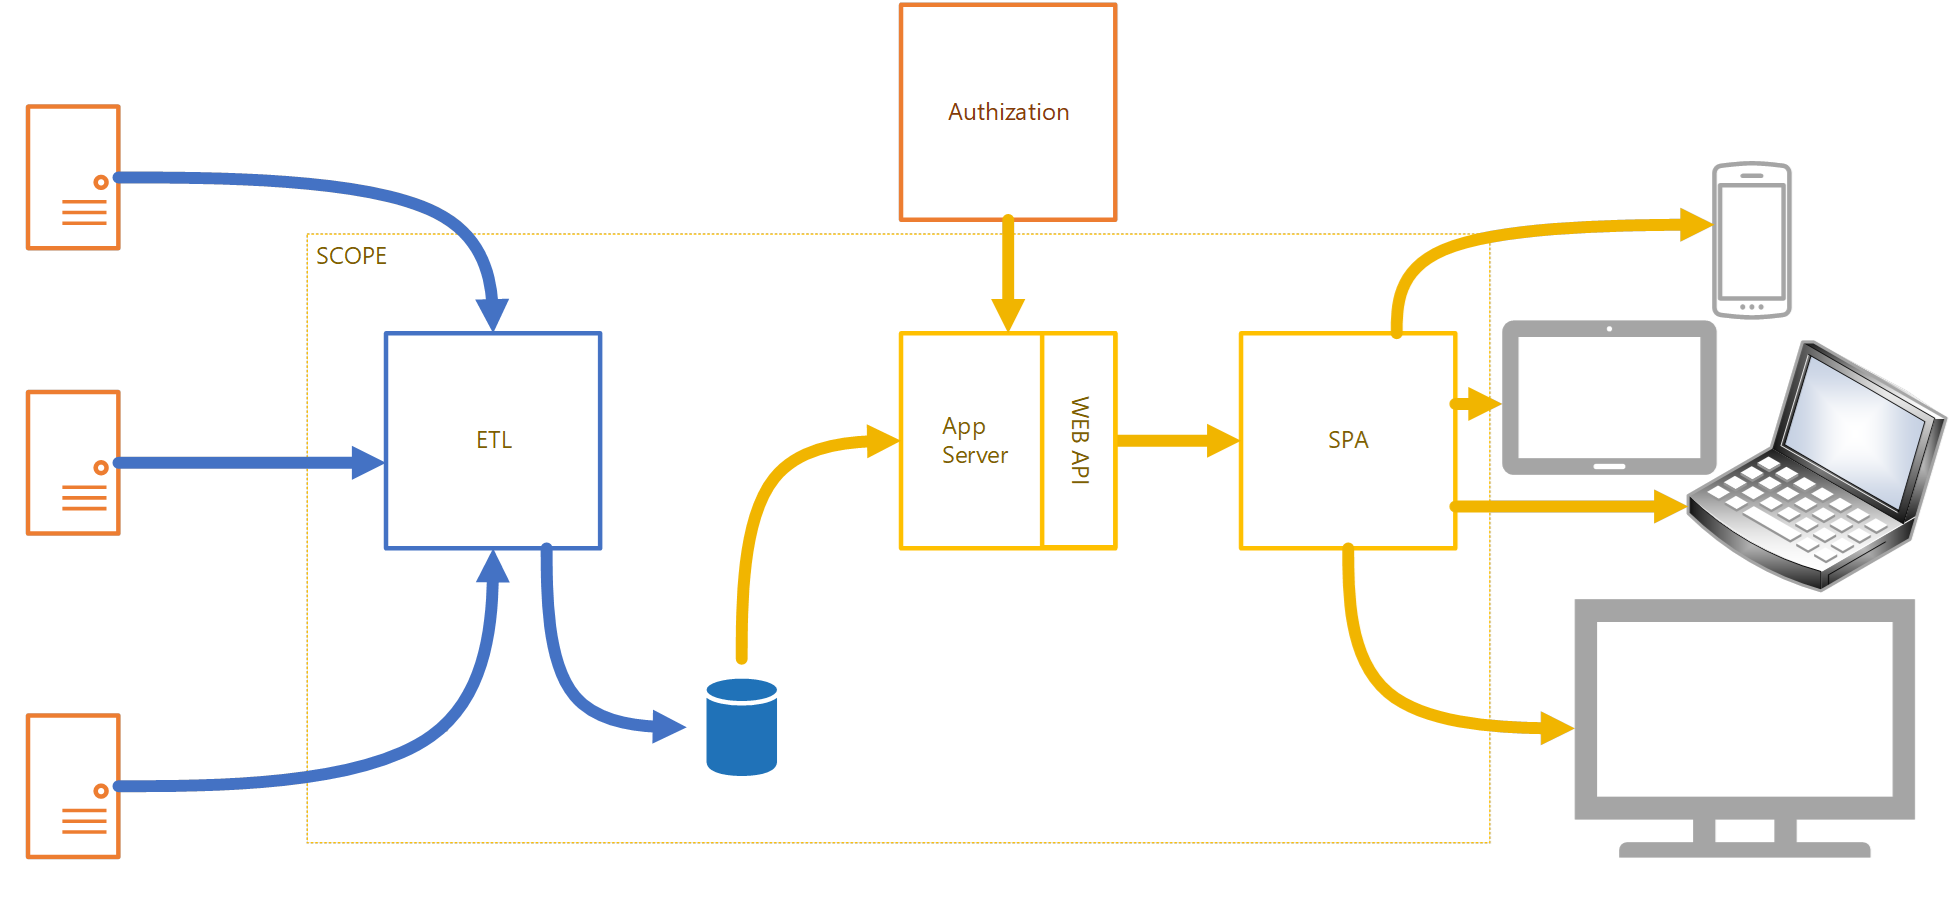
\includegraphics[width=\textwidth]{lean-dashboard-software-architecture.png}
\end{center}

This figure depicts the various components of our application interacting with each other.
\newline
The rightmost part of the figure represents the information sources. These sources provide its users with an Application Programming Interface (API), this API will be used by the  ETL to obtain solely the needed information.
\newline
This information can take different forms. The data objects received from the APIs will differ in terms of structure and information, for example, a project is different from an issue. This means it is crucial to implement an optimized Extract module within the ETL component of our application.
\newline
After extracting this information, the ETL will send it towards its respective Transformation module, where it will be treated and converted into a new data object with the necessary fields to represent it visually later.
\newline
The Load module of the ETL will grab this newly created Widget object and load it on a database.
\newline
The ETL procedure is constantly running and updating the existing widgets on the database, according to the widget's time settings that will be presented in this document.
\newline
In the middle of the scheme is the core of the application, the Web Server, and its API.
\newline
The Web Server is responsible for processing the requests that will be sent by the Single Page Application (SPA), as well as managing the NoSQL database running on ElasticSearch\cite{ES}.
\newline
It interacts with an authorization and authentication module, the Authization module, to manage the users and their roles within the application.
\newline
The API supports a varied range of operations that can be called by the user to manipulate the information inside the database. It presents the user with methods to obtain, create, update, and delete the information in the database.
\newline
Lastly on the rightmost side of the diagram, there is the SPA, the component that will be accessed by the application user on their preferred device.
\newline
To provide the user with the best experience, this SPA will be developed as a mobile-first, responsive web application capable of supporting different types of display screens, starting from the smartphone up to the bigger ones like a regular desktop computer or a TV screen.

\section{Scheme of the back-end}
\begin{center}
    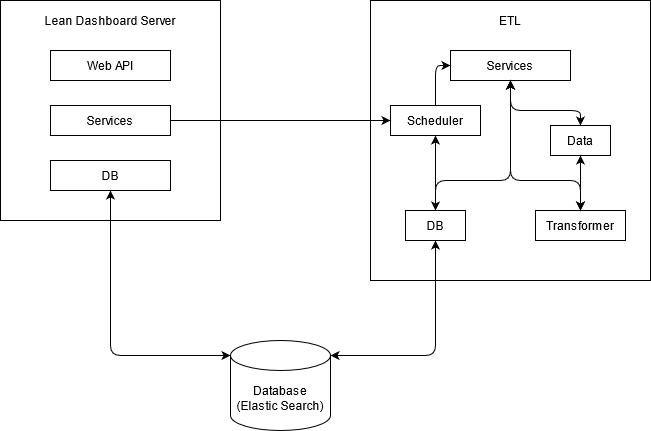
\includegraphics[width=\textwidth]{arquitetura software.png}
\end{center}
The back-end of the Lean Dashboard application is made of two key components, the Web Server(Lean Dashboard Server) and the ETL.
\newline
These two components interact with one another so that the ETL knows what sort of information it should obtain.
\newline
The Lean Dashboard Server is composed of 3 Node.JS\cite{NODE} modules:
\begin{itemize}
  \item The Web API module is responsible for catching the requests sent to the API, filtering the parameters and body fields, and sending them to the Services module.
  \item The services module will process every request the Web API receives and forms a function call to the Database(DB) module. If the request consists of modifying or creating a Widget object it will make a call towards the Scheduler module in the ETL.
  \item The DB module is responsible to access and modify the ElasticSearch based database, containing all the necessary functions to create, obtain, delete and edit the database. It also verifies if the inputted parameters are valid within the context of the application, preventing the existence of duplicates or the association of members to a project who aren't registered in the application, for example.
\end{itemize}
The ETL component, as we already mentioned, is responsible for accessing the various data sources and transforming them into a specific widget object.
\newline
It contains 5 Node.JS modules in its structure:
\begin{itemize}
  \item The Scheduler module, accessed by the lean-Services module, is responsible for scheduling the automatic ETL process that will update the created widgets according to the time settings a user provides. It accesses the DB module to retrieve the necessary information to execute the correct Services function.
\newline
The module is implemented using the node-cron\cite{NODECRON} module so that we can easily create and configure jobs to execute at a set time.
It contains 2 Map objects with distinct functionalities, the widgetMap is responsible for providing the scheduler with the necessary ETL-Services function to execute for the various widgets according to the function parameter contained within the widget's structure, and the widgetJobs associates a widgetId to its currently running job so that we can reconfigure them at a later date.
  \item The ETL-Services module acts as a coordinator for the ETL procedure, it obtains the necessary filtered data from the Data module and then gets the transformed information from the Transformer module.
\newline
After the process of obtaining information is complete it calls the DB module so that this information can be stored.
  \item The Data module's task is accessing the selected information sources, currently Azure, Jira, and Squash, and sending them to the Transformer module for some light filtering, returning the retrieved object with only the necessary information for its transformation.
  \item The Transformer module's job is to transform the data into the required information for the widget to be displayed. Currently, it transforms the data into widgets such as a Pie Chart, a Data Table, or a Gauge Chart.
  \item Finally, the DB module is responsible for updating the widget's information with the updated data obtained from the ETL procedure.
\end{itemize}

\newpage
\section{Data Model}
For the Data model and the storage of the information, we chose the No-SQL database Elastic Search.
\\ \newline
To better facilitate the getting and storage of information, we divided each object into they're own index, as displayed in the following scheme:
\begin{center}
    \resizebox{120mm}{!}{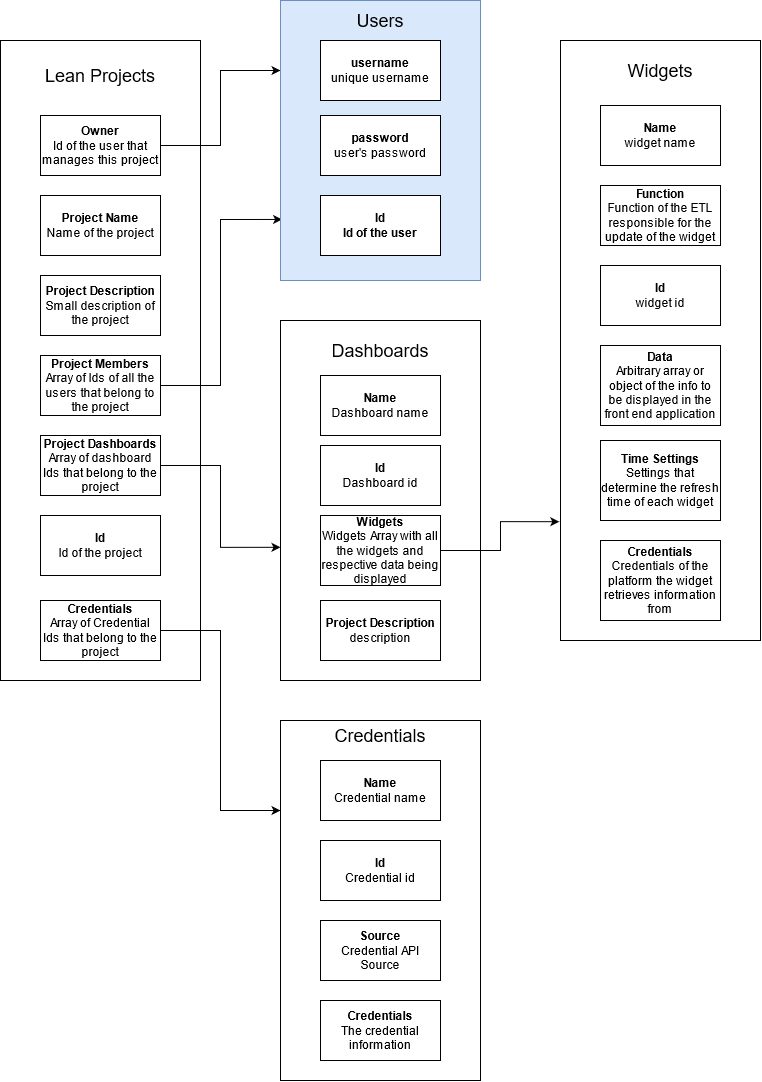
\includegraphics[width=\textwidth]{modelo de dados.png}}
\end{center}
\textbf{Lean Projects}
\newline
This is the index where all the Projects created with our application will be stored, acting as the main gatherer of information.
\newline
It has information over who created it (Owner), the Project's name, its description, and a unique identifier.
\newline
Each project can contain a varied number of members, dashboards, and credentials. 
\newline
This information is stored inside an Array of identifiers, these being Project Members for the members that are currently associated with the project, Project Dashboards for the dashboards, and Credentials for the credentials.
\newline
The members simply act as viewers of the information within the project, they can only access dashboards and view the information on the widgets.
\newline
\newline
\textbf{Users}
\newline
The users are highlighted in a different color on the scheme to better differentiate them from the data model since they aren't being stored in the database our application manages and are being stored in the Authization module's database.
\newline
Each user will have a username and a password so they can log in to our application, as well as a unique identifier within the database to be used by the array of members within the Lean Projects Objects.
\newline
\newline
\textbf{Dashboards}
\newline
The dashboards are where the widgets will be stored. They don't exist if there isn't at least an already existing Lean Project and will be presented as a web page with all the widgets within the dashboard being displayed.
\newline
The dashboard objects contain a name, an Array of Widget identifiers that are associated with the dashboard, a description, and a unique identifier within the database.
\newline
\newline
\textbf{Credentials}
\newline
The credentials consist of a specific object containing a name, a source (Azure, Jira, or Squash), and a credential object containing all the credentials themselves.
\newline
This credential object is structured as such for each of the information sources:
\newline
\begin{center}
    \resizebox{120mm}{!}{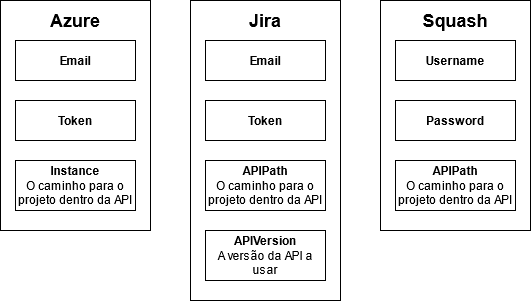
\includegraphics[width=\textwidth]{formato das credentials.png}}
\end{center}
Each source requires a different form of credential so that the authentication on their web API is successful. These credentials are mandatory as the ETL procedure cannot access the specified information source's API without them.
\newline
Azure requires an email, a token, and an Instance field related to the project within the API.
\newline
Jira requires an email, a token, an APIPath for the project within the API, and an APIVersion that refers to the API version to be used.
\newline
Squash only requires a username, a password, and the APIPath.
\newline
\newline
\textbf{Widgets}
\newline
The widgets are the result of the ETL procedure.
\newline
They are created by the user through the selection of a widget template that will serve as a widget with temporary data to be displayed.
\newline
Widgets are made out of several fields like a name, a function, a data object, the time settings for the ETL schedule, the required credentials, and a unique identifier.
\newline
The function field refers to which ETL function the scheduler needs to call to start the node job.
\newline
The time settings are an object that contains information related to the interval at which the ETL procedure is executed to update the widget. 
\newline
Each field of this object is structured in CronTab format and consists of:
\begin{itemize}
  \item seconds;
  \item minutes;
  \item hours;
  \item day of the month;
  \item month;
  \item day of the week;
\end{itemize}
The credentials are the credential object associated with the project.
\newline
Without them obtaining information is impossible, making it a required field when creating the widget.
\newline
The data object is where all the transformed ETL information will be stored. It is the main reason the application utilizes an ElasticSearch database, as the information contained within this object will vary from widget to widget, making it a hard task to store consistently within a relational database like PostgreSQL.


\newpage
\section{Authization module, Backoffice and Access control}
 To give our users authorization and authentication features we had to think of a way of letting users create accounts, have users with different roles inside the application and have different roles have their privileges. To give users that set of features, and as a request of Inetum, we utilized a Node module called Authization\cite{AUTHIZATION}. 

As a reference point, this module was a project developed last year by the ISEL students Tiago Matias, Diogo Leandro andJoão Barata of the LEIC programme as a final project of the Project and Seminar course, and was also developed in partnership with Inetum, and serves as a module that allows to set up an RBAC model with various roles, permissions and decide which roles should have access to what permissions. The module will also take care of aspects such as login, logout and the creation of users. Since the module requires a SQL Database for the storage of users, we had to use  PostgreSQL\cite{POSTGRESQL} to handle the storage of users, the created roles and permissions.

As for the RBAC model, it was requested that there were three types of users: a master user, with every kind of accesses and ultimate control (that includes access to every existing project, both seeing and editing them), a user that would be able to manage certain projects and create new ones and finally a user with only permission to see projects he is a part of.
With that said, we came up with an RBAC model with the roles Superuser, Manager and Collaborator, with the following accesses:
\\ \newline

\begin{center}
    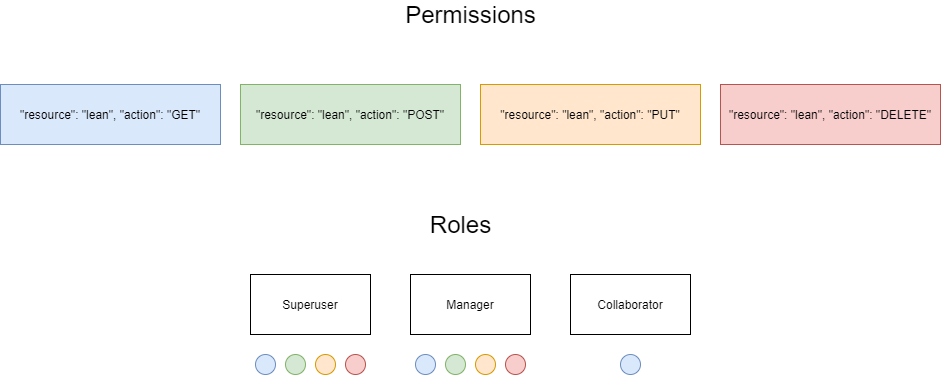
\includegraphics[width=\textwidth]{lean-rbac-model.png}
\end{center}

As said before, we defined three roles. The Superuser will have access to all of the defined permissions, being able to access and modify all projects,  without having to be a part of them. 
Below the Superuser, the Manager role will act in a similar way to the Superuser, but will only be able to modify projects that we're created by himself. Additionally, he will only be able to visualize projects (and the dashboards and widgets associated with the said project) if he is a member or instead, the creator of that project. A manager will be able to manage aspects of a project such as its name, description, containing dashboards and widgets, as well as all the members in it.
Finally, the role of Collaborator. Being the role with fewer permissions, users with this role will only be able to access projects they are members of.

\chapter{User Experience Research}
User Experience, commonly called UX, is the term used when referring to how users interact with a certain product. If we use an analogy, if we were to open a door, it is more about how the door handle is used than what shape or colour it has, or what material it is made from. 

UX is also greatly impacted by the context a product is being used and the type of users using said product. With the guidance provided by Inetum, one company member provided us with a list of personas. That list of personas would help us take into consideration how we would address the UX design of our early digital prototypes (which later reflect on the client application), by having various types of users with specific personalities, most wanted features and specific positions inside a company. 

Following that, we developed a digital prototype that would allow us to make a series of usability tests with real users. Those tests would allow us to better determine what needed to be addressed in our digital prototype and solve issues before any implementation was being done.

With that said, we believe the User Experience research done by the group is something that can greatly improve the result of the client application, whilst saving implementation time by allowing us to make some decisions beforehand. Usually, problems are easier to solve in a digital prototype than they are in code.

\section{Red routes diagram}
A  Red Routes matrix is developed to aid a designer to identify the crucial and frequent tasks which users perform with our product. It consists of a matrix that delivers the frequency of performing,  as well as the number of users who perform a specific task.
\\ \newline
In the process of identifying Red Routes, there are some factors to be considered:
\begin{itemize}
	\item  Critical: Tasks that deliver relevant value to users
 	\item Frequency: Tasks there are performed at high frequency, usually represent the use cases of over 90\% of users.
 	\item Key-value drivers: Red Routes drive the key business metrics
 	\item  Impact: Red Routes affects significantly the overall user experience
\end{itemize}
Through identification of our users' top tasks, we can:
\begin{itemize}
	\item Foresee users' needs
	\item Develop a website utilizing users' needs
	\item Target fundamental website pages
	\item Conduct usability tests
\end{itemize}	
Regarding the identification of Red Routes' major advantage, it aids the team to identify the most important content and functionality rooted in usefulness to most users.  Further, it supports a team in the selection of the minimum viable product (MVP), which leads to a more significant product roadmap design with the purpose of continuous iteration and overcome potential usability barriers on relevant user journeys. 
\begin{center}
    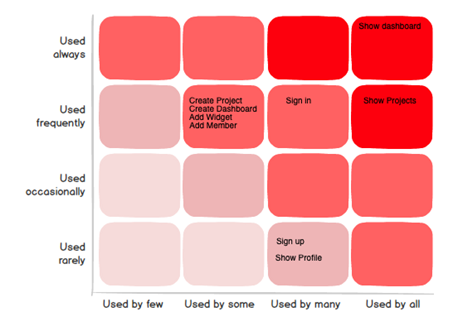
\includegraphics[width=\textwidth]{red-routes-diagram.png}
\end{center}
\newpage

\section{Information Architecture}
To better organize and structure the flow and various paths of our web application, we made our Information Architecture schema using the platform Miro:
\\ \newline
\begin{center}
    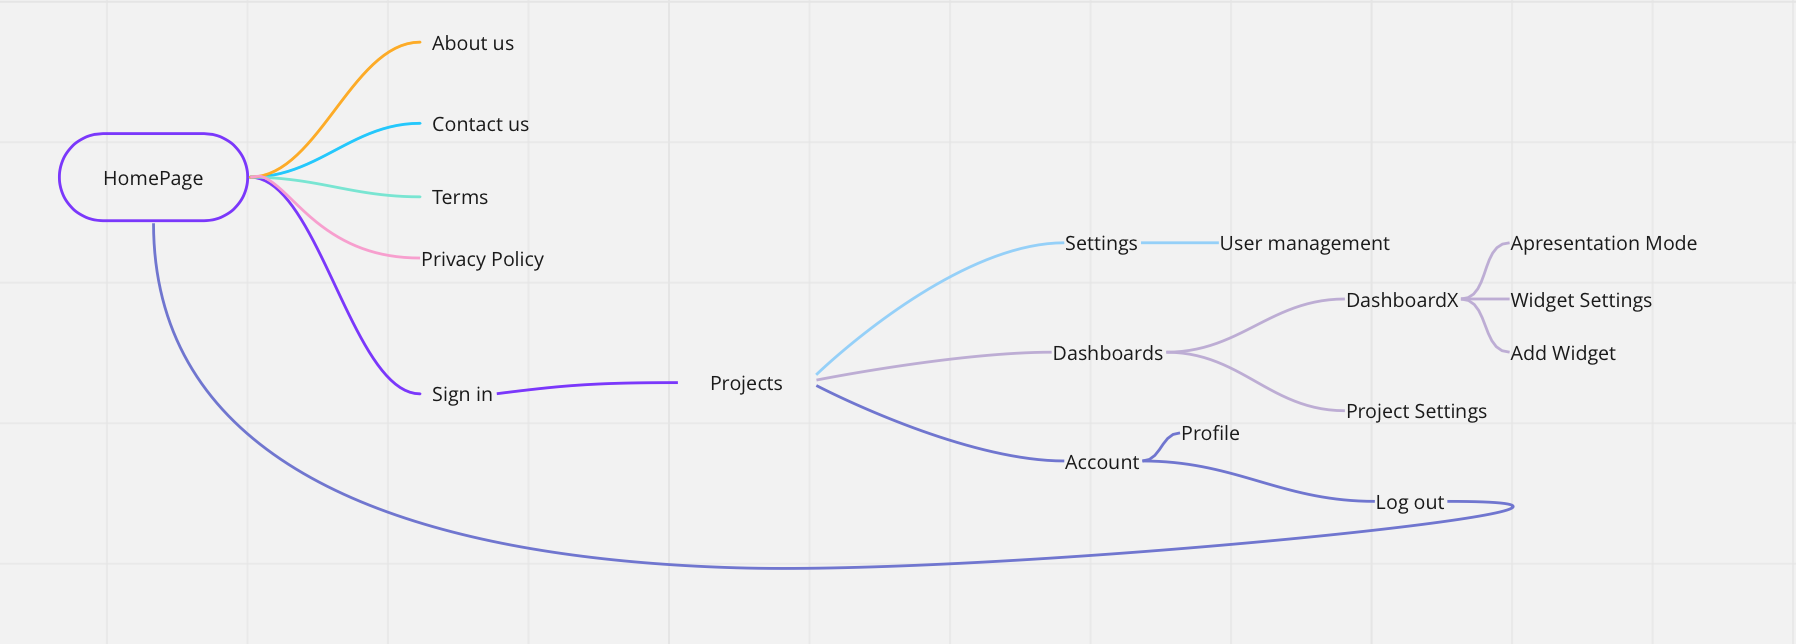
\includegraphics[width=\textwidth]{information-architecture.png}
\end{center}

With this diagram, we can better plan the making to the various resources by achieving a flowchart that dictates if the various flowchart accesses make sense (and easily correct them if they don't)

\section{Digital Prototype}
A Digital Prototype is a tool used in UI research to develop a mock user interface that can be utilized in use-case tests. These tests gather a small group of people and establish a task that all users need to complete. 
\\ \newline
A Digital Prototype is how we validate our basic idea and the premises underpinning it by collecting user feedback.
With the obtained results, we can then determine what aspects need to be addressed in the Digital Prototype by us developed.
\\ \newline
This research and planning done beforehand (before the full implementation of the client application) can greatly decrease implementation costs since it is much easier to make modifications to this mocked user interface than it is to make some of the same changes on the client application code.
We utilized the platform Figma\cite{FIGMA} to develop our Digital Prototype, this being the prototype obtained:
\\ \newline
\begin{center}
    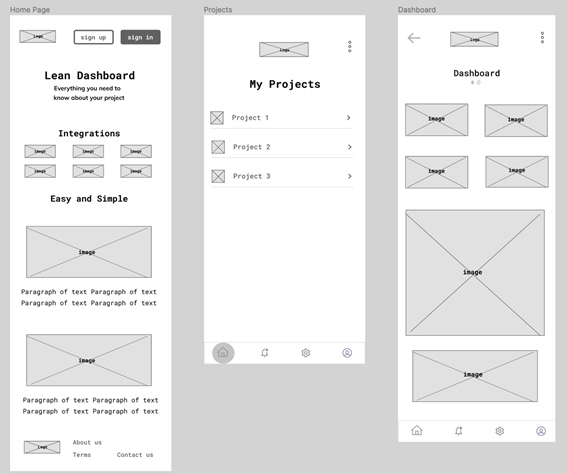
\includegraphics[width=\textwidth]{digital-prototype.png}
\end{center}

\chapter{Client Application}
*Nesta secção iríamos explicar alguns príncipios da aplicação cliente, bem como mostrar algumas das páginas por nós já feitas*

\begin{thebibliography} {websites}

\bibitem{INETUM} Inetum\\ https://gfi.world/pt-en/

\bibitem{ETLPROC} ETL - Understanding It and Effectively Using It.\\
https://medium.com/hashmapinc/etl-understanding-it-and-effectively-using-it-f827a5b3e54d\\
Consulted on April 1st 2021

\bibitem{AUTHIZATION} Authization Module\\
https://github.com/dleandro/Authentication-and-Authorization-Node-Component-

\bibitem{POSTGRESQL} PostgreSQL: The World's Most Advanced Open Source Relational Database\\
https://www.postgresql.org/

\bibitem{MIRO} Miro - Platform used for the Information Architecture schema\\
https://miro.com/

\bibitem{REACT} React\\ https://reactjs.org/

\bibitem{FIGMA} Figma Prototype tool\\https://www.figma.com/prototyping/

\bibitem{ES} ElasticSearch \\ https://www.elastic.co/elasticsearch/

\bibitem{NODE} Node.JS \\ https://nodejs.org/en/

\bibitem{NODECRON} node-cron \\ https://www.npmjs.com/package/node-cron
\end{thebibliography}

\end{document}